\documentclass[12pt,a4paper]{article}
\usepackage{ctex}
\usepackage{amsmath,amscd,amsbsy,amssymb,latexsym,url,bm,amsthm}
\usepackage{epsfig,graphicx,subfigure}
\usepackage{enumitem,balance}
\usepackage{wrapfig}
\usepackage{mathrsfs,euscript}
\usepackage[usenames]{xcolor}
\usepackage{hyperref}
\usepackage[vlined,ruled,commentsnumbered,linesnumbered]{algorithm2e}

\newtheorem{theorem}{Theorem}
\newtheorem{lemma}[theorem]{Lemma}
\newtheorem{proposition}[theorem]{Proposition}
\newtheorem{corollary}[theorem]{Corollary}
\newtheorem{exercise}{Exercise}
\newtheorem*{solution}{Solution}
\newtheorem{definition}{Definition}
\theoremstyle{definition}


%\numberwithin{equation}{section}
%\numberwithin{figure}{section}

\renewcommand{\thefootnote}{\fnsymbol{footnote}}

\newcommand{\postscript}[2]
{\setlength{\epsfxsize}{#2\hsize}
	\centerline{\epsfbox{#1}}}

\renewcommand{\baselinestretch}{1.0}

\setlength{\oddsidemargin}{-0.365in}
\setlength{\evensidemargin}{-0.365in}
\setlength{\topmargin}{-0.3in}
\setlength{\headheight}{0in}
\setlength{\headsep}{0in}
\setlength{\textheight}{10.1in}
\setlength{\textwidth}{7in}
\makeatletter \renewenvironment{proof}[1][Proof] {\par\pushQED{\qed}\normalfont\topsep6\p@\@plus6\p@\relax\trivlist\item[\hskip\labelsep\bfseries#1\@addpunct{.}]\ignorespaces}{\popQED\endtrivlist\@endpefalse} \makeatother
\makeatletter
\renewenvironment{solution}[1][Solution] {\par\pushQED{\qed}\normalfont\topsep6\p@\@plus6\p@\relax\trivlist\item[\hskip\labelsep\bfseries#1\@addpunct{.}]\ignorespaces}{\popQED\endtrivlist\@endpefalse} \makeatother

\usepackage{listings}

\begin{document}
\noindent

%========================================================================
\noindent\framebox[\linewidth]{\shortstack[c]{
\Large{\textbf{Homework07}}\vspace{1mm}\\
CS214-Algorithm and Complexity, Spring 2018}}
\begin{center}

\footnotesize{\color{black} Name: 杨培灏  \quad Student ID: 516021910233}
\end{center}

\begin{enumerate}

\item 设计算法判定平面上n个点是否在一条直线上
\begin{solution}
	根据输入点的坐标,如果他们的横坐标$x$均相同,则必然在一条直线$x=x_0$上。否则根据两点可以建立直线方程,检查其余点是否在该直线上。
	\begin{algorithm}
		\caption{onTheLine()}
		\KwIn{点集V,点有x,y属性}
		\KwOut{各点是否在一条线上}
		\If{$v_1.x=v_2.x$}{
			\For{$v \in V$}{
				\If{$v\ne v_1$}{
					直接返回 False;
				}
			}
			直接返回 True;
		}
		\For{$v \in V$}{
			$a=(v_2.y-v_1.y)/(v_2.x-v_1.x)$;\\
			$b=v_1.y-a\times v_1.x$;
		}
	\end{algorithm}
	\textbf{复杂度分析:}遍历各点检查坐标及其横坐标x对应的直线函数的函数值,所以为$\mathcal{O}(n)$。
\end{solution}

\item 设P是包围在给定矩形R中的一个简单多边形,q为R中任意一点,设计高效算法寻找连接q和R外部一点的线段,使得该线段与P相交的边的数量最少

\begin{solution}
	首先判断点q是否在多边形P内部,如果q在P内部,那么无论如何取点,都会与P有且仅有一个交点。当它不在P内部时,该点在P与R之间。那么在取R外部的点时,该线段与P的交点情况可以用如下方式判断:q与P的顶点组成的直线(即支撑线)的夹角最大和最小的情况下是一个交点,在该夹角间的线段均为在判断是否在P内部时求出的count大小,该夹角外部一个则交点也没有。可以用下面两个图表示。
	\begin{center}
		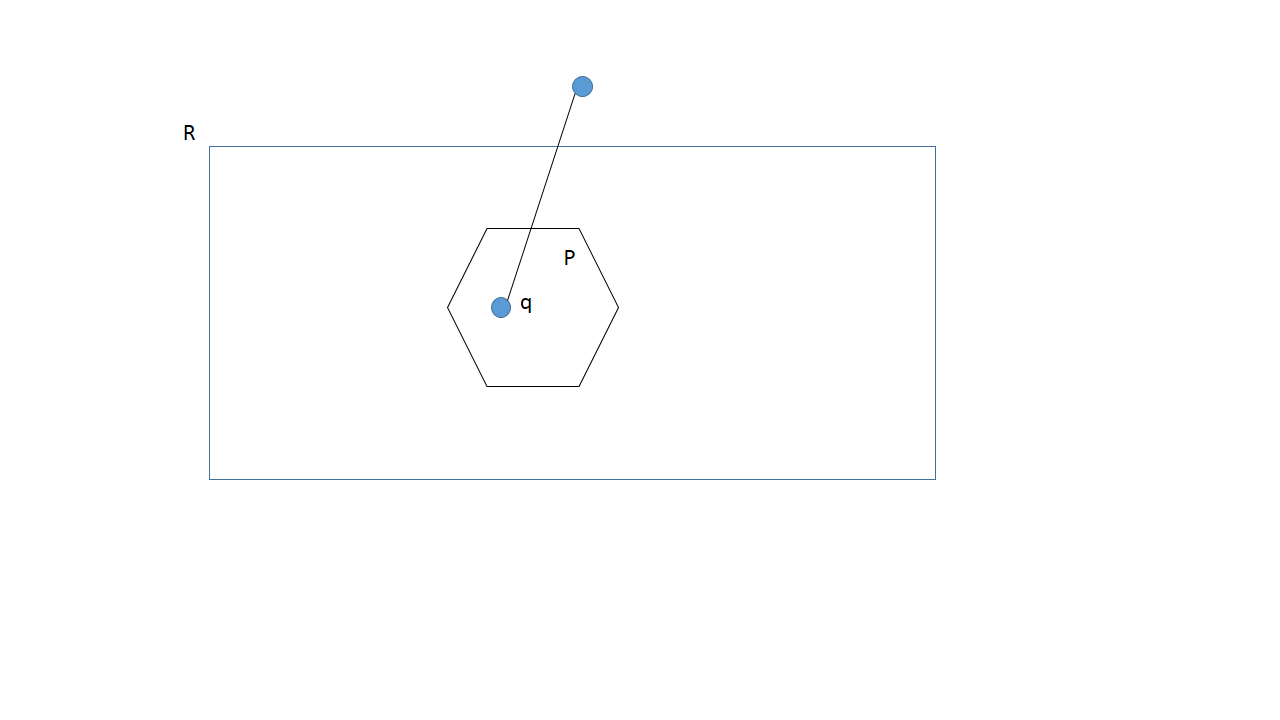
\includegraphics[width=0.75\textwidth]{figure1.PNG}
	\end{center}
	\begin{center}
		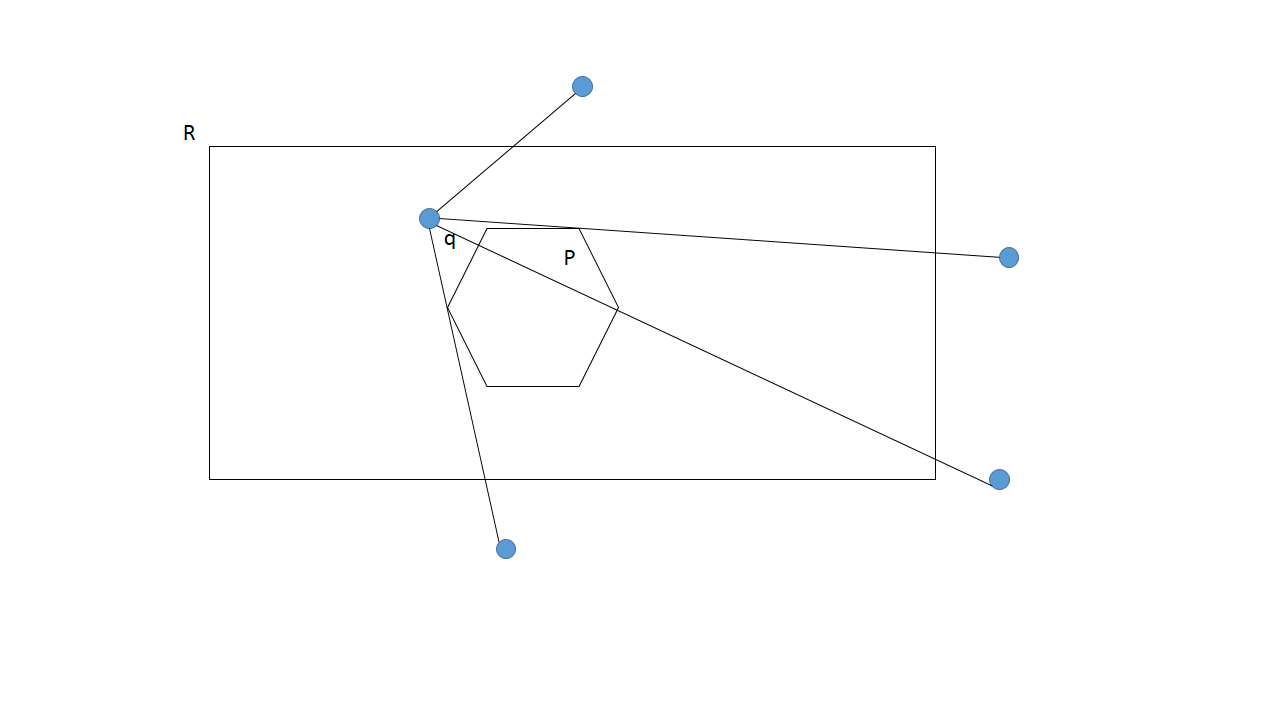
\includegraphics[width=0.75\textwidth]{figure2.PNG}
	\end{center}
	\begin{algorithm}
		\caption{findLeastEdge()}
		\KwIn{点$q$坐标$q.x$和$q.y$,多边形$P$的各顶点$V_p={p_1,...,p_n}$,边为$E_p={e_1,...,e_n}$}
		count=0;
		\For{$all edges e_i of the polygon$}{
			\If{$the line x=x_0 intersects e_i$}{
				//假设该交点不是多边形的顶点并且直线$x=x_0$与$e_i$不重合\\
				求出$y_i$是$x=q.x$and多边形P的边$e_i$交点的纵坐标\\ 
				\If{$y_i <q.y$}{
					count=count+1;
				} 
			}
		}
		//判断是否在P内部\\
		\If{count为奇数}{
			Inside=true;//在P内部\\
			直接返回之前的count值\\
		}\Else{
			inside=false;
		}
		\If{inside=false}{
			取直线$x=q.x$,$\forall i\in{1,2,...,n}$,记直线$-q-p_i-$与它的夹角(与y轴负方向,取为角度起始,逆时针增大)为$\alpha_i$,其最大值最小值记作$\beta$和$\gamma$。
			那么R外的点v只要满足-q-v-与$x=q.x$所成角度不在$\beta$和$\gamma$间即可与该多边形无交点。
		}
	\end{algorithm}
	\textbf{复杂度分析:}最坏情况下,需要首先确定点q是否在P的内部,该算法的时间复杂度为$\mathcal{O}(n)$。接下来遍历多边形P的各顶点,得到它们与点q组成的支撑线的角度关系,该过程的时间复杂度为$\mathcal{O}(n)$。所以算法的时间复杂度为$\mathcal{O}(n)$。
\end{solution}

\item 给定平面上一组点,求该点集的直径。(文献查阅,然后用自己的语言进行算法思想的描述,包括时间复杂性分析)
\begin{solution}
	该方法基于一个定理:点集中最远的点对一定在凸包上。那么我们可以先求出凸包,之后利用旋转卡壳法求解点集的直径。求解凸包的算法是首先对各点根据相对极端点的角度排序,排序后对前$k$个点求解凸路径,之后加入第$(k+1)$个点,求新加入的点与凸路径最后一段的角度(该角度从凸路径内侧测量),如果小于$180^{\circ}$,则说明连接上该点仍为凸路径,否则去掉凸路径中最后一段,再次连接。旋转卡壳法则利用了对踵点,凸包上的顶点位于两条平行切线上则为对踵点。最大直径只可能在对踵点间,同时在逆时针旋转选择不同顶点时,其对踵点也在逆时针旋转变化,不可能在上一顶点的对踵点的顺时针方向。对踵点最多有$3n/2$对。求解凸包的时间复杂度为$\mathcal{O}(n\log n)$,之后旋转卡壳法的时间复杂度为$\mathcal{O}(n)$,总的时间复杂度为$\mathcal{O}(n\log n)$。
	\begin{algorithm}
		\caption{maxDistance}
		\KwIn{输入点集$P={p_1,\ldots,p_n}$}
		\KwOut{点集直径}
		首先选定点$p_1$为极端点,其$x$值最大,当有多个点$x$坐标相同时,取$y$坐标值最小的一个。
		\For{$i=2\to n$}{
			计算$-p_1-p_i-$与$x$轴的夹角$\alpha_i$;
		}
		根据$\alpha_i$对P中的点排序;\\
		//以上为排序部分\\
		$q_1=p_1$;\\
		$q_2=p_2$;\\
		$q_3=p_3$;\\
		m=3;
		\For{$i=4\to n$}{
			\While{$-q_m-q_m-$和$-q_m-p_k-$间夹角$\geq180$}{
				m=m-1;
			}
			m=m+1;
			$q_m=p_k$;
		}
		//以上为求解凸包部分得到凸包的顶点集合$Q={q_1,\ldots,q_n}$\\
		从凸包顶点集Q中取出两极端点$q_{min}$和$q_{max}$;\\
		通过两点建立平行线,这两点是一对踵点,计算两点间距;\\
		旋转平行线,直到其中一条与凸包某边重合,那么得到了新的踵点;\\
		以该边一端点替换之前的踵点中的点,找到了新的一对踵点;\\
		重复上面两步直至回到$q_{min}$和$q_{max}$;\\
		计算两点间距即可;\\
		//以上为根据凸包应用旋转卡壳法\\
	\end{algorithm}
\end{solution}

\item 在平面上给定一个有$n$个点的集合$S$,求$S$的极大点。极大点的定义:设$p_1=(x_1,y_1)$和$p_2=(x_2,y_2)$是平面上的两个点,如果$x_1\le x_2$并且$y_1\le y_2$,则称$p_2$支配$p_1$,记为$p_1\prec_2$。点集$S$中的点$p$为极大点,意味着在$S$中找不到一个点$q$,$q\ne p$并且$p\prec q$,即$p$不被$S$中其它点支配。
\begin{solution}
	首先取$x$值最大的点记作$P_1(x_1,y_1)$(如果有多个点$x$相同最大值,那么取$y$值最大的一个,显然直线$y=y_1$下方的点均不可能为极大点。再取$y$值最大的点为$P_n(x_n,y_n)$(多个相同最大$y$值的点时取$x$值最大的一个,显然直线$x=x_n$左侧的点均不可能为极大点。极大点只可能出现在$P_1$和$P_n$确定的矩形范围内。如果$P_1=P_n$,那么只有一个极大点$P_1$。否则,显然$(x_1,y_n)$点是不存在的,那么可以对矩形区域内部的各点,先根据x值排序,从$P_1$开始向$x$的负方向遍历,相同横坐标点取纵坐标最大的一个,并记录当前的最大的$y$值,新的遍历到的点的$y$值不能比该值低。这样时间复杂度为$\mathcal{O}(n\log n)$。
	\begin{algorithm}
		\KwIn{$n$个点集合$S$}
		\KwOut{极值点计数counter}
		遍历一次S,确定两个极端点,其x和y值分别最大,记为$P_1$和$P_2$;\\
		\If{$P_1=P_2$}{
			直接返回 counter=1;\\
		}\Else{
			根据x值排序以$P_1$和$P_2$为对角顶点的矩形区域内的点得到有序的T。
			$ymax=y_1$;\\
			counter=2;\\首先$P_1$和$P_2$肯定是极大点。
			\For{$s\in T$ and$s.x=x_1\to x_2$}{
				\If{yMax>y}{
					跳过该点;\\
				}\Else{
					counter=counter+1;\\
				}
			}
		}
	\end{algorithm}
\end{solution}
\end{enumerate}

%========================================================================
\end{document}
